\documentclass{standalone}
% translate with >> pdflatex -shell-escape <file>

% This file is an extract of the PGFPLOTS manual, copyright by Christian Feuersaenger.
% 
% Feel free to use it as long as you cite the pgfplots manual properly.
%
% See
%   http://pgfplots.sourceforge.net/pgfplots.pdf
% for the complete manual.
%
% Any required input files (for <plot table> or <plot file> or the table package) can be downloaded
% at
% http://www.ctan.org/tex-archive/graphics/pgf/contrib/pgfplots/doc/latex/
% and
% http://www.ctan.org/tex-archive/graphics/pgf/contrib/pgfplots/doc/latex/plotdata/

\usepackage{pgfplots}
\usepackage{pgfplotstable}
\pgfplotsset{compat=newest}

% The manual loads these libraries globally; the extracted standalone examples
% need them too. external/clickable/snakes are intentionally omitted.
\usetikzlibrary{
	arrows.meta,backgrounds,calc,decorations.footprints,decorations.markings,
	decorations.pathreplacing,fixedpointarithmetic,intersections,patterns,
	plotmarks,shapes.arrows,spy,through}
\usepgfplotslibrary{
	colorbrewer,colormaps,dateplot,fillbetween,groupplots,patchplots,polar,
	smithchart,statistics,ternary,units}

% Some colormap examples reuse this display style defined earlier in the manual.
\pgfplotsset{
	cycle from colormap manual style/.style={
		x=3cm,y=10pt,ytick=\empty,
		colorbar style={x=,y=,ytick=\empty},
		point meta min=0,point meta max=1,
		stack plots=y,
		y dir=reverse,colorbar style={y dir=reverse},
		every axis plot/.style={line width=2pt},
		legend entries={0,...,20},
		legend pos=outer north east,
	},
}

\pagestyle{empty}

\begin{document}
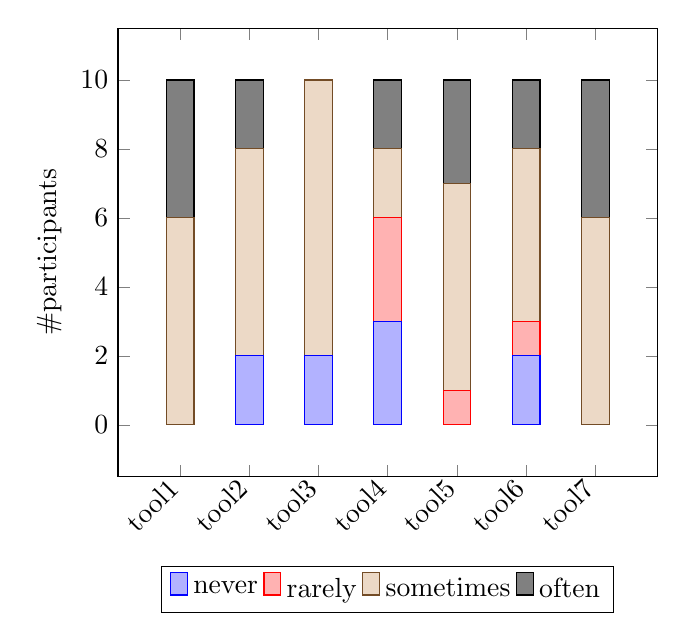
\begin{tikzpicture}
\begin{axis}[
    ybar stacked,
    enlargelimits=0.15,
    legend style={at={(0.5,-0.20)},
        anchor=north,legend columns=-1},
    ylabel={\#participants},
    symbolic x coords={tool1, tool2, tool3, tool4,
        tool5, tool6, tool7},
    xtick=data,
    x tick label style={rotate=45,anchor=east},
]
\addplot+ [ybar] coordinates {(tool1,0) (tool2,2)
  (tool3,2) (tool4,3) (tool5,0) (tool6,2) (tool7,0)};
\addplot+ [ybar] coordinates {(tool1,0) (tool2,0)
  (tool3,0) (tool4,3) (tool5,1) (tool6,1) (tool7,0)};
\addplot+ [ybar] coordinates {(tool1,6) (tool2,6)
  (tool3,8) (tool4,2) (tool5,6) (tool6,5) (tool7,6)};
\addplot+ [ybar] coordinates {(tool1,4) (tool2,2)
  (tool3,0) (tool4,2) (tool5,3) (tool6,2) (tool7,4)};
\legend{never, rarely, sometimes, often}
\end{axis}
\end{tikzpicture}
\end{document}
